\documentclass[10pt]{jarticle}
%% 高さの設定
\setlength{\textheight}{\paperheight}   % ひとまず紙面を本文領域に
\setlength{\topmargin}{-5.4truemm}      % 上の余白を20mm(=1inch-5.4mm)に
\addtolength{\topmargin}{-\headheight}  % 
\addtolength{\topmargin}{-\headsep}     % ヘッダの分だけ本文領域を移動させる
\addtolength{\textheight}{-40truemm}    % 下の余白も20mmに
%% 幅の設定
\setlength{\textwidth}{\paperwidth}     % ひとまず紙面を本文領域に
\setlength{\oddsidemargin}{-5.4truemm}  % 左の余白を20mm(=1inch-5.4mm)に
\setlength{\evensidemargin}{-5.4truemm} % 
\addtolength{\textwidth}{-40truemm}     % 右の余白も20mmに

\usepackage{ascmac} 
\usepackage[dvipdfm]{graphicx}
\usepackage{scala}

\begin{document}
\begin{screen}
この1〜2年、開発者のコミュニティなどで 着実に人気が高まっているプログラミング言語が「Scala(スカラ、スケーラと読みます)」 です。本特集では、Javaプログラマ(見習いも含みます)に向けて、Scalaをなるべく簡潔にわかりやすくお伝えします。  
\end{screen}

Scalaは、スイス連邦工科大学ローザンヌ校のMartin Odersky(マーティン・オーダスキー)教授率いるチームが開発しているプログラミング言語です。オープンソース(BSDライセンスに似たSCALA LICENSE)で開発・公開されており、その範囲内で自由に利用できます。最初に、“なぜ、 Scalaの人気が高まっているのか”を説明します。


\section*{オブジェクト指向と関数型の特徴を備える} 
Scalaは、オブジェクト指向に加えて関数型言語の特徴を備えた比較的新しい言語です。この、“オブジェクト指向に加えて”というのがポイントです。新しいパラダイム(問題解決のための考え方)を、従来のパラダイムに重ね合わせていることから、マルチパラダイムの言語ともいわれます。 ちなみにScalaという名前は、Scalable Language(拡張性のある言語)の短縮形です。そのスケーラブルという言葉には、「小さいプログラムも大規模なプログラムも同じ概念で記述できるべきである」という、柔軟性や拡張性を重視した言語設計の意図が込められています。 Scalaは、関数型言語の機能を取り込むことで、簡潔で明瞭なコーディング、言語自体の拡張性、バグを作り込みにくいプログラミングスタイル、並行処理向きなど、オブジェクト指向とは異なる特徴を持っています。簡潔な表現の一例として、同じ機能のクラスをScalaとJavaで書いたコードをソースコード1に示します。 

\begin{lstlisting}[label=src:money, caption=お金を表すクラスのScala版とJava版]
// Scala版
package money
import java.util.Currency

// amountはお金の量, currencyは通貨単位    
class Money(val amount : BigDecimal, val currency : Currency)    
 
// Java版
public class Money {
  private final BigDecimal amount;
  private final Currency currency;
  public Money(BigDecimal amnt, Currency creny) {
    amount = amt;
    currency = creny;
  }
  public BigDecimal getAmount() {
    return amount;
  }
  public Currency getCurrency() {
    return currency;
  }
}
\end{lstlisting}
\section*{Javaの資産を生かせる}
ソースコード\ref{src:money}では通貨の単位を表すjava.util.Currnecyが利用されています。Scalaは実行環境にJava仮想マシン(Java VM)を利用するため、ScalaプログラムからJavaの機能をシームレスに利用することができるのです。このようにJavaとの親和性が高いのも大きな特徴です。Javaプログラマにとっては、オブジェクト指向の知識を生かしつつ関数型言語の考え方をスムーズに取り入れながら、Javaの資産も利用できるわけです。 こうして見てくると、JavaプログラマがScalaに注目するのも当然のように思えてきませんか。Scalaは、Javaプログラマが次に学ぶに値する言語です。より品質の高いプログラムを書けるようになるためにScalaの知識はきっと役立ちます。早速、開発実行環境を整備して、Scalaのプログラミングスタイルを見ていきましょう。
\part{統合開発環境の整備}
まずは、Scalaの開発環境をPCにインストールしましょう。前提条件を表1にまとめましたのでお手元のPCのシステム環境を確認しておいてください。例えば、図1に示すコマンド(java -version)を実行することにより、Javaのバージョンが確認できます。 

\begin{table}[htb]
  \caption{Scalaの開発環境をPCにインストールするときの前提条件}
  \begin{center}
    \begin{tabular}{|l|c|r||r|} \hline
      JDK7以上をインストールしてあること\\ \hline
      JDKのインストールパスをJAVA\_HOMEとして環境変数に登録してあること\\ \hline
      \$JAVA\_HOME/binを環境変数のPathに追加してあること\\ \hline 
    \end{tabular}
  \end{center}
  \label{tb:table1}
\end{table}

\section{Scala配布ファイルのダウンロードと展開}
それでは、Scala本体をインストールします。「Scala Distribution - The Scala Programming Language (http://www.scala-lang.org/downloads)」のWebページから最新版であるscala-2.9.2.final.zip(2012年7月上旬現在) をダウンロードします。そして、scala-2.9.2.final.zipを任意のディレクトリ(フォルダ)に展開します。
\section{環境変数を設定する}
ScalaをインストールしたディレクトリをSCALA\_HOMEとして環境変数に設定します。さらに、\$SCALA\_HOME/binをPATHに追加します(表2)。 本体のインストールはこれだけで終了です。以下のコマンドを実行してバージョン番号などが表示されれば正しく導入できています。

\begin{verbatim}
$ scala -version
Scala code runner version 2.9.2 -- Copyright 2002-2011, LAMP/EPFL
\end{verbatim}

\section{IntelliJ IDEAを使ってみよう}
次に、Scalaプログラミングに使える代表的な統合開発環 境の一つ、「IntelliJ IDEA」をインストールしてみましょう。 IntelliJ IDEAは、チェコ共和国に本社を構えるJetBrains社が提供するJava用の統合開発環境です。 有償の製品ですが、Apacheライセンスを採用したオープンソース版 「Community Edition」も用意されており、商用/非商用を問わず無償で利用できます。このIntelliJ IDEAにScala用のプラグインを追加することで、Scalaプログラミングが可能です。Eclipseでも同様にScalaプログラミングが可能ですが、現時点では動作の安定性でIntelliJ IDEAが勝ると思います。(インストール手順については別掲記事を参照)。

\section{Scala対応プロジェクトを作成する}
早速、IntelliJ IDEAを使ってScalaプログラムを動かして みましょう。文法についてはこの後の基礎編で説明します。 メニューから「File」→「New Project」を指定してくださ い。New Projectのウィザードが表示されます。「Create project from scratch」が選択されている状態で「Next」を クリックしてください。 図2のようなプロジェクト名(Name:)やプロジェクトを配置するディレクトリ(Project files location:)、プロジェクトの形式(Create module)などを選択する画面が表示されます。プロジェクトの形式は通常、「Java Module」を選択します。 次に、ソースディレクトリを作成するか否かを 指定する画面が表示されます。特に問題なければ、 「Create source directory」を選択して「Next」 をクリックしてください。続いて開いた画面で、どのプラグインを有効にするかを 選択します。ここでは、「Scala」を選びます。Scala Settingsの「Use Scala distribution」は、 SCALA\_HOMEが指定されていれば、そのパスが設定されているはずです。指定されていなければ手動で設定します。

\begin{figure}[hb]
  \centering
  \caption{プロジェクトの設定}
  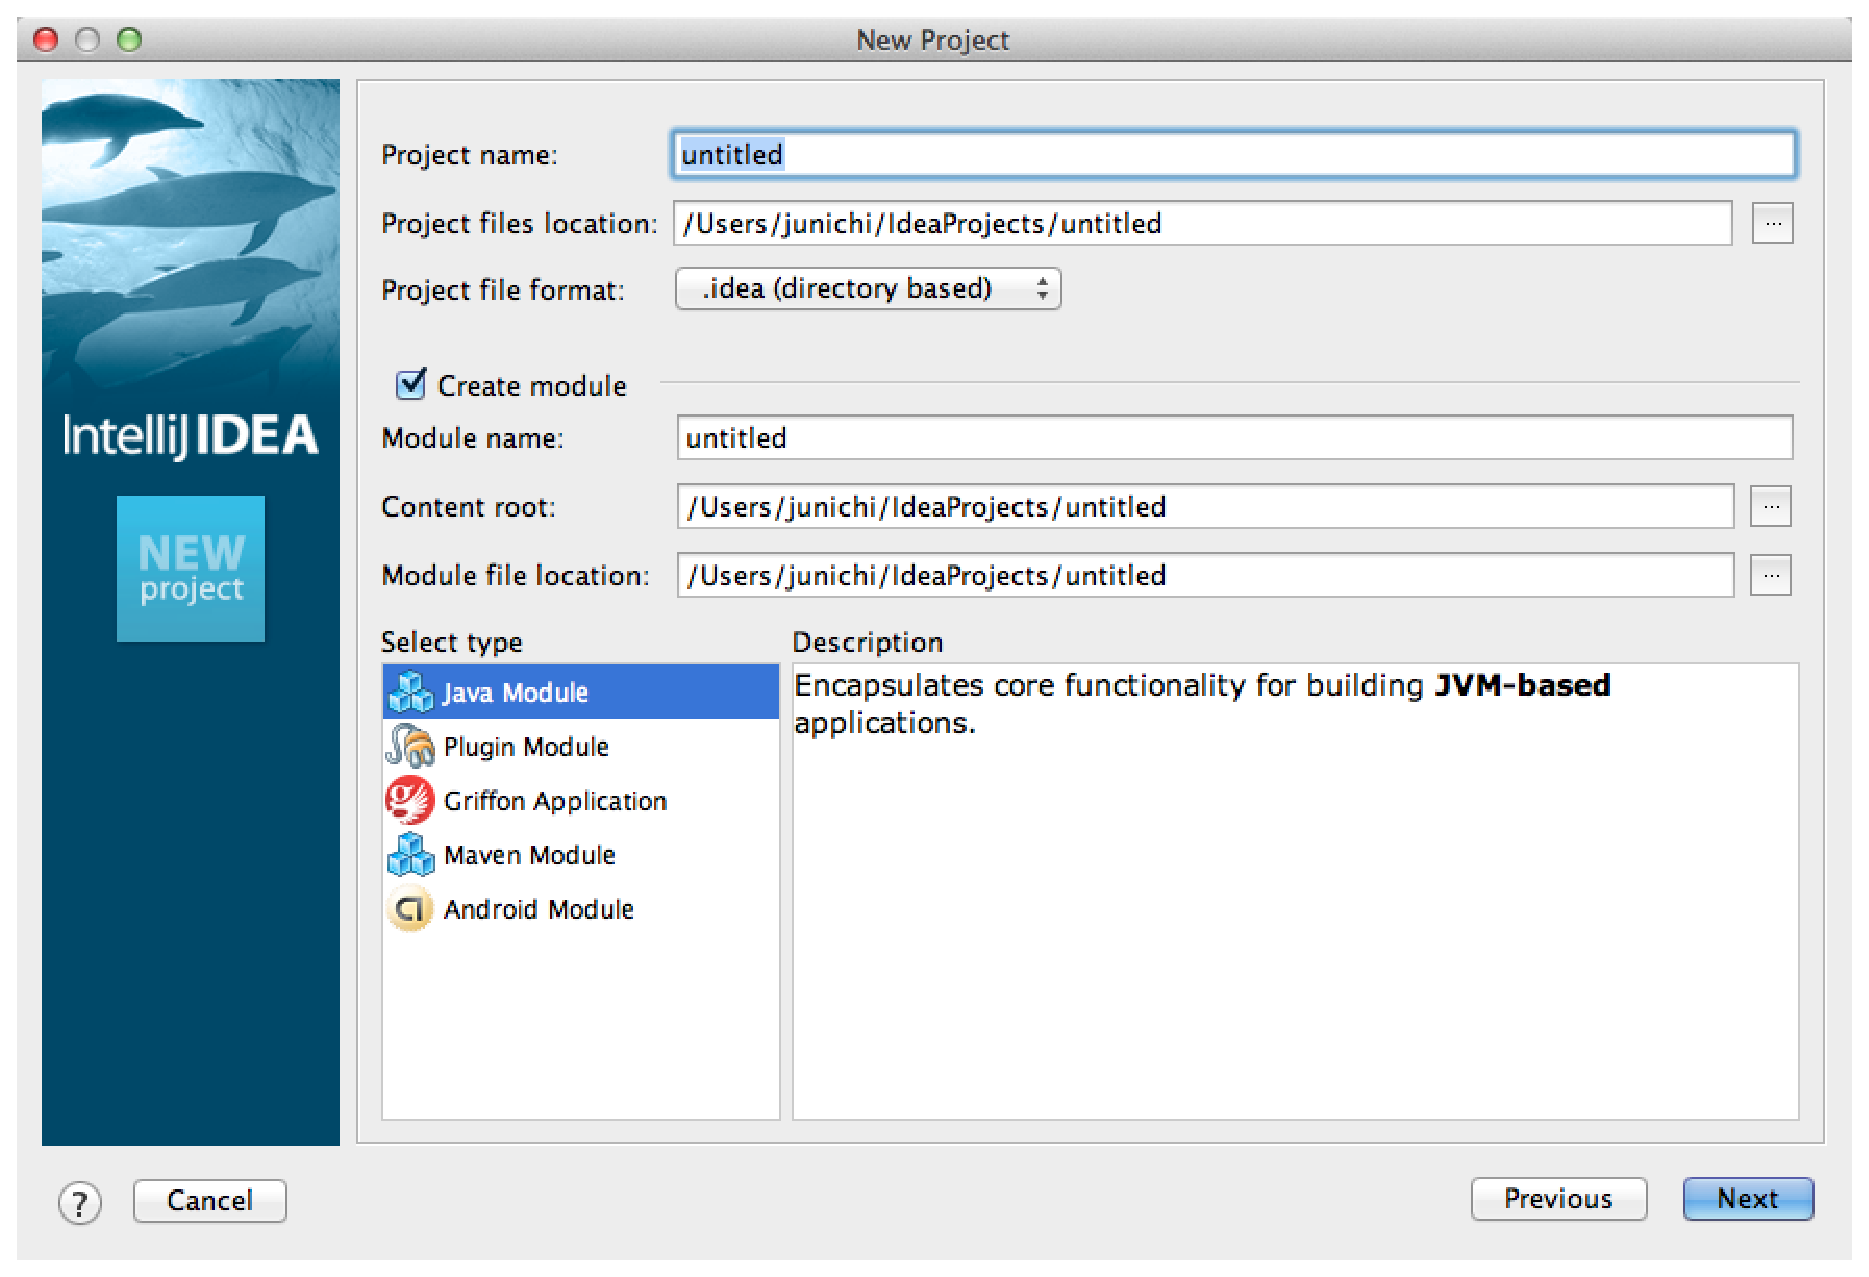
\includegraphics[scale=0.5]{img/new_project.eps}
\end{figure}

\begin{figure}[hb]
  \centering
  \caption{オブジェクトの作成}
  
\includegraphics[scale=0.5]{img/create_new_scala_class.eps}
\end{figure}

\begin{lstlisting}[label=src:helloworld, caption=HelloWorld.scala]
object HelloWorld {
  def main(args:Array[String]):Unit = {
    println("Hello, World!")
  }
}
\end{lstlisting}

\section{クラスを作ってビルド・実行する}
それでは、ビルドとプログラムの実行を試しましょう。簡 単なプログラム例としてHello, World!を表示するプログラム を作成します。 前述の手順で作成したプロジェクトでsrcフォルダに HelloWorldオブジェクトを作成します。後述するように、オ ブジェクトは特別なクラスです。srcディレクトリを右クリッ クして、「New」→「Scala Class」を選択し、開いたウィンド ウでHelloWorldのObjectを作成します(図3)。 HelloWorldオブジェクトのコードがリスト2です。ここで は「HelloWorld.scala」と表示されたエディタ領域にこのま ま入力してください。 HelloWorldオブジェクトを含むプロジェクト全体をビルド するには、メニューから「Build」→「Make Project」を指定 します。HelloWorldオブジェクトだけをコンパイルするには「Build」→「Compile 'HelloWorld.scala'」をクリックします。 それでは、IntelliJ IDEA上で実行してみましょう。 HelloWorldオブジェクトにカーソルがある状態で、メニューの「Run」→「Run」をクリックして、プログラムを実行します。 Hello, World!という表示がIntelliJ IDEAのコンソールに表 示されるはずです(図4)。デバッグをしたい場合には、「Run」 →「Debug」を指定します。 Eclipseユーザーのために、Eclipseのショートカットを併 記したIntelliJ IDEAの代表的なショートカット一覧を表3 に示します。

\part{一目でわかる「HelloWorld」}
ここで、Scalaプログラムの実行方法を整理しておきましょう。Scalaには、以下の三つの実行方法があります。 
\setcounter{section}{0}

\section{対話型インタプリタで実行する}
最初は、Scalaのコードをインタプリタで対話的に実行する方法です。この実行環境のことをREPL(Read Eval Print Loop)といいます。コマンドラインからscalaコマンドを実行するとREPLが起動し、「\verb|scala>|」というプロンプトが表示されます。このプロンプトに続けて、Scalaのプログラムを入力してEnterキーを押すと、実行結果が対話的に確認できます。 
\begin{verbatim}
scala> println("Hello, World!")
Hello, World!
\end{verbatim}
REPLは「:quit」あるいは「:q」と入力してEnterキーを押すと終了します。

\begin{itembox}[l]{Scalaのセミコロン}
Javaでは文の最後にセミコロン(;)が必要ですが、Scalaでは 1行に一つの文を記述する場合はセミコロンを省略できます。ただし次のように、1行に複数の文を記述する場合は必要です。
\begin{verbatim}
val message = "Hello, World!"; println(message)
\end{verbatim}
\end{itembox}

\section{スクリプトモードで実行する}
Scalaのプログラムをスクリプトとして実行する方法です。まず、中身が次の1行だけの「HelloWorldScript.scala」というスクリプトファイルを作成してください。
\begin{lstlisting}
println("Hello, World!")
\end{lstlisting}
そのスクリプトファイルを次のようにして実行します。
\begin{verbatim}
$ scala HelloWorldScript.scala
Hello, World!
\end{verbatim}
実行する際、Windowsが警告を出す場合があります。その場合はアクセスを許可してください。 
\section{コンパイル済みのプログラムを実行する}
Javaと同様にコンパイラによってコンパイルしたプログラムを実行する方法です。まず、コンパイルの対象となるソースコードを用意します。そして、scalacコマンドでこのソースコードをコンパイルします。
\begin{verbatim}
$ scalac HelloWorld.scala
\end{verbatim}
コンパイルされたプログラムをscalaコマンドで実行します。
\begin{verbatim}
$ scala HelloWorld
Hello, World!
\end{verbatim}
最後に、HelloWorld.scalaに基づいて、Scalaの文法を紹介します。詳しくは次ページ以降で説明しますので、ここでは気楽に図6を見てください。このHelloWorld.scalaを Javaで記述したのが、見慣れたHelloWorld.javaです。
\end{document}
